\newcommand{\fngitrouterconfigscript}{%
	\footnote{The RT configuration script for setting IP routes, speed, and RTT of the connections is available in  \url{https://github.com/reisdout/git-udt/blob/main/scripts/config_router.sh}}%
}

\vspace{-3cm}

\begin{figure}[h!t]
	\centering
	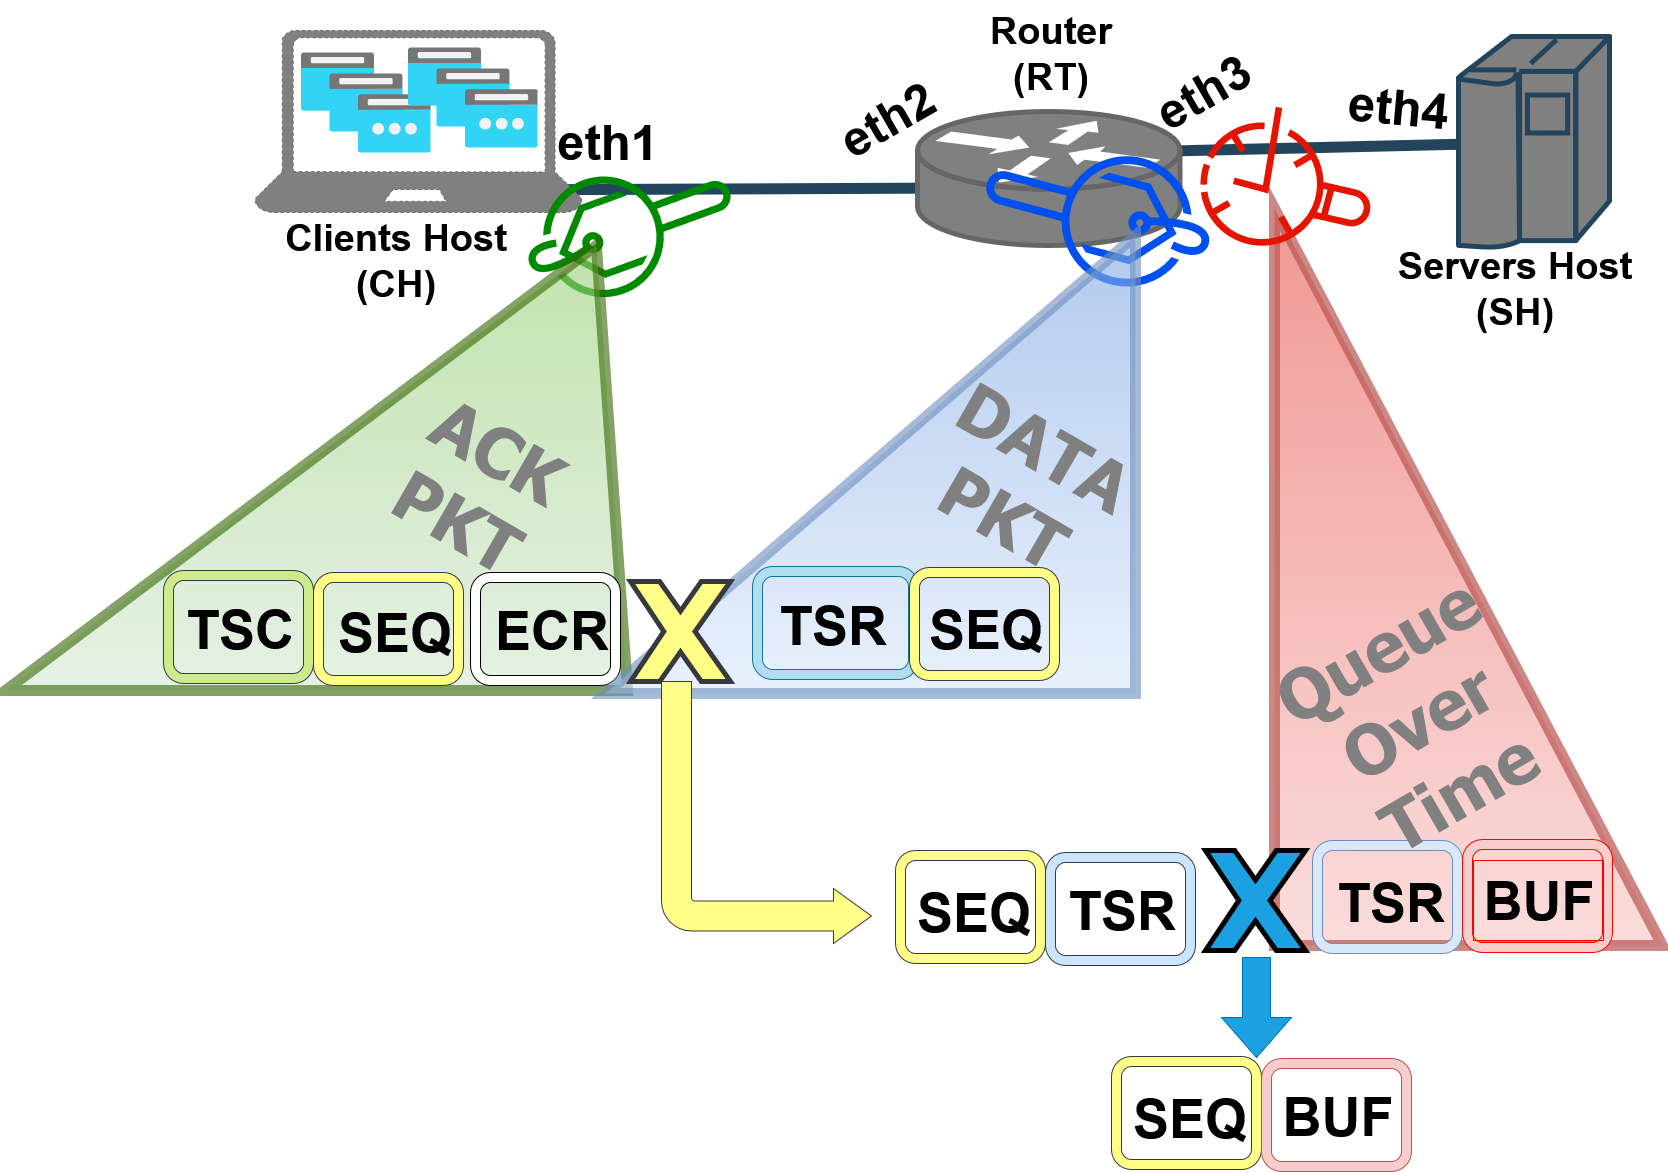
\includegraphics[width=0.6\textwidth]{figure_0006.png}
	%\caption{}
	\label{fig:dumbell_poc}
\end{figure}    


\begin{table}[h]
	\centering
	\caption{Configuration of PoC setup machines.}
	%\centering
	\begin{tabular}{|c|m{0.9\linewidth}|}		\hline
		Machine & \hspace{0.4\linewidth}Spec \\ \hline
		Clients Host (CH) & \textbf{OS}: Linux Mint 22 x86\_64; \textbf{Kernel}: 6.8.0-38-generic; \textbf{CPU}: 12th Gen Intel i7-12700H (20) @ 4.600GHz; \textbf{Memory}: 3050MiB / 64052MiB; \textbf{Ethernet interface}: RTL8125 2.5GbE Controller -vendor: Realtek Semiconductor Co., Ltd. \\
		& \\
		Router (RT) & \textbf{OS}: Linux Mint 22 x86\_64; \textbf{Kernel}: 6.8.0-52-generic; \textbf{CPU}: Intel Atom C2758 (8) @ 2.400GHz; \textbf{Memory}: 1015MiB / 7912MiB; \textbf{Ethernet interface}: Ethernet Connection I354 - vendor: Intel Corporation \\
		&\\
		Servers Host (SH) & \textbf{OS}: Linux Mint 22 x86\_64; \textbf{Kernel}: 6.8.0-38-generic; \textbf{CPU}: 11th Gen Intel i7-1165G7 (8) @; \textbf{Memory}: 1347MiB / 15790MiB; \textbf{Ethernet interface}: RTL8111/8168/8211/8411 PCI Express Gigabit Ethernet Controller - vendor: Realtek Semiconductor Co., Ltd. \\ \hline
	\end{tabular}	
	\label{tab:poc_setup_machines_spec}
\end{table}

